\documentclass[conference]{IEEEtran}
\IEEEoverridecommandlockouts
% The preceding line is only needed to identify funding in the first footnote. If that is unneeded, please comment it out.
\usepackage{cite}
\usepackage{amsmath,amssymb,amsfonts}
\usepackage{cite}
\usepackage{algpseudocode}
\usepackage{graphicx}
\usepackage{textcomp}
\usepackage{xcolor}
\usepackage{amsthm}
\usepackage{algorithm}
%\usepackage{algorithmic}
\usepackage{epstopdf}
\usepackage{subfigure}
\usepackage{verbatim}
\usepackage{diagbox}

\newcommand{\tabincell}[2]{\begin{tabular}{@{}#1@{}}#2\end{tabular}}
\def\BibTeX{{\rm B\kern-.05em{\sc i\kern-.025em b}\kern-.08em
    T\kern-.1667em\lower.7ex\hbox{E}\kern-.125emX}}
\begin{document}

\title{Workload-Aware Scheduling for Heterogeneous-Storage Data Analytics\\
}

\author{\IEEEauthorblockN{name1, name2, name3, and name4}
\IEEEauthorblockA{State Key Lab. for Novel Software Technology, Nanjing University, CN\\
Email: email address, \{email address\}@nju.edu.cn}}


\maketitle
%Since the read speeds of diverse storage devices are quite different, the unbalanced use on either specific type of storage or particular device would easily overload them, making them being hotspots and finally worsen the read performance for analytical tasks.
\begin{abstract}
A trend in nowadays data centers is that equipped with SSD, HDD, etc., heterogeneous-storage devices are widely deployed to meet different demands of various big data workloads. Since the read speeds of diverse storage devices are quite different, the unbalanced use on either specific type of storage or particular device would easily elongate the latency on reading data, worsening the overall performance for analytical tasks. In this paper, we formulate Workload-Aware Scheduling problem for Heterogeneous-storage (WASH), as well as show its NP-hardness. To solve this proposed problem, we design a randomized algorithm (WASH-rdm) which chooses source devices based on delicate calculated probabilities and can be proved concentrated on its optimum with high probability through our theoretical analysis. Extensive experiments show that the WASH-rdm can reduce the reading time for tasks by up to 55\% over the state-of-the-art baseline algorithm.

\end{abstract}

\begin{IEEEkeywords}
big data analytics, heterogeneous-storage, workload-aware scheduling
\end{IEEEkeywords}

\section{Introduction}

Nowadays, there are new trend that data centers have a variety of data analytical workloads, e.g., some data streaming applications like Storm
\cite{b40} and other machine learning based applications like Grep \cite{b27}. The different workloads might have different requirements on storage performance \cite{b28} \cite{b29} \cite{b30} \cite{b31}. For example, Storm is a compute-intensive application whose computation relies significantly on the I/O performance while Grep is a I/O-intensive application which has a great throughput on I/O. In order to meet these demands, a lot of heterogeneous devices have been deployed in big data analytics frameworks, e.g., Hadoop \cite{b14} and Spark\cite{b15}.

However, the heterogeneity of these devices would lead to the divergent read performance due to two aspects. Firstly, the different types of storage, e.g. SSD \cite{b32} and HDD \cite{b33}, have different read performance, naturally. For example, as shown in Fig.\ref{Fig:motivation} reading the same amount of data from HDD takes almost twice longer than SSD. Secondly, when there are a large number of tasks reading data concurrently from specific device, read performance is also affected. As further shown in Fig.\ref{Fig:motivation}, when the amount of tasks increases, the reading time for each task will also increase.

Due to the different read performance, traditional scheduling may result in unbalanced usage on storage device. For example, when tasks fetch data from those disks with high-performance, they would spend less time on I/O, compared with those low-performance disk. Furthermore, the I/O queries containing too many data analytical tasks may easily overload the storage devices. As a result, disks with poor read performance or heavy workload would elongate the I/O performance of analytical tasks.

\begin{figure}[!t]
	\centering
	\includegraphics[height=1.8in]{fig_motivation5.eps}
	\caption{Comparisons of (1) reading time for one piece of data with unified size, i.e., 64MB, on various storage. (2) reading time for various I/O workloads.}
	\label{Fig:motivation}
\end{figure} 

%However, due to the divergent read performance of different storage and the cumulative workload of the storage, its hard to hard to achieve this aim. 
 
Thus, we propose to focus on dealing with unbalanced use of heterogeneous-storage devices in this paper. However, due to the multiple replicas of data, how to choose these feasible locations is a big challenge.
 Most of the researches focus on heterogeneous computing resources \cite{b25}\cite{b26}\cite{b35}\cite{b36}, ignoring the heterogeneous-storage devices. Although some works have already considered heterogeneous-storage \cite{b6}\cite{b7}, multiple types of storage are not considered. In contrast, we formulate the Workload-Aware Scheduling problem for Heterogeneous-storage as well as prove its NP-hardness. Afterwards, we propose a randomized algorithm (WASH-rdm) with guaranteed performance by carefully choosing source device based on delicate calculated probabilities.
%We focus on two aspects. One is the read performance of the disk itself, the other is the load of the disk, that is, the number of tasks that are reading the data from the disk. Focus on the above two points, we formulate it as an optimization problem and propose a heuristic algorithm (WASH-greedy) and a random algorithm (WASH-rdm) with guaranteed performance to solve the problem. %Experiments show that the performance of the proposed algorithm is 55\% better than the Storage-unaware scheduling mechanism. 
More concretely, our contributions are as follows: 

\begin{itemize}
%\item We present the necessity of sloving this problem by showing impact of reading data phase during the task execution.
\item To balance the workload on heterogeneous-storage device, we propose Workload-Aware Scheduling problem for Heterogeneous-storage (WASH) which is proved to be NP-hard. 
\item We propose randomized algorithm with guaranteed-performance. The WASH-rdm algorithm can be proved concentrated around its optimum with high probability 1 - O($e^{-t^2}$) where $t$ is the concentration bound.
\item The results of our extensive simulations show that the performance of our proposed WASH-rdm improves by up to 55\% over the art-of-the-state algorithms.
%compared with the storage-unaware scheduling mechanism and by 20\% 
\end{itemize}

The rest of the paper is organized as follows. In Section \ref{RELATED_WORKS}, we present the related works of the WASH problem. Then we propose our system model and our algorithm in Section  \ref{SYSTEM_MODEL} and Section  \ref{DESIGN_ALGORITHM}. At last, we conclude this paper in Section \ref{CONCLUSION} by summarizing our main contributions.


\section{RELATED WORKS}\label{RELATED_WORKS}
The related works consist of two parts. For the first part, due to limited link bandwidth, some works focus on data locality to improve data analytics performance. However, in heterogeneous environments, it is not enough to consider data locality alone. Thus, some other studies have been carried out to accelerate data analytical tasks by studying hardware heterogeneity \cite{b1}.

Due to the limited network bandwidth resources in data center, while a large amount of data is transmitted between nodes before task execution, it will greatly affect the data analytics. Therefore, processing data locally as much as possible can improve performance, e.g., placing map task to the node which stores the input data. Matei et al. \cite{b2} proposes delay scheduling to assure data locality. Delay scheduling considers that when a node has idle slots, priority should be given to  the tasks whose input data is stored at that node, and delay to schedule tasks whose related data is not stored at that nodes. Ganesh \cite{b3} makes multiple replicas for high-frequency data by analyzing the access frequency of data, improving the data locality in this way. Cristina \cite{b4} proposes a distributed adaptive data replication algorithm DARE, which can help the scheduler show better data locality. Jalaparti \cite{b5} believes that most of the production work is repetitive and predictable, by which the scheduler could make scheduling plan ahead. Coordinating the tasks and data placement of these jobs can effectively reduce bandwidth usage, further, improving data locality. All of these work improves the performance of data analytics by improving data locality.

However, in heterogeneous data centers, due to the different performance of data storage devices, task reading time is often different. At present, some of the existing work is based on the research of storage heterogeneity, which accelerates the speed of data processing. Xu et \cite{b6} considers the current usability of underlying hardware (CPU, memory, I/O), but does not consider the performance differences of different storage hardware. 
In Hadoop 2.8, HDFS\cite{b19} considers heterogeneous-storage and supports multiple storage strategies. One of the storage strategies is ONE\_SSD, that is, one replicas is stored in SSD, and the rest is stored in HDD. However, the task scheduling strategy is not aware of the disk's performance.
Based on ONE\_SSD, Pan \cite{b7} proposes H-Scheduler which takes into account the performance between HDD and SSD. Facing the trend of increasing heterogeneous-storage, it is one-sided to divide the storage devices into two categories. Wang B \cite{b8} uses Markov model to describe the use of nodes in the cluster to deploy data reasonably. However, the scheduling problem of tasks is not considered, and the heterogeneity of different storage media is also not considered. These work does not accurately define the differences between storage hardwares, and there is still a situation where a large number of tasks read low-speed devices, causing bottlenecks.

The difference between those tasks and ours is that our work specificly defines the difference in reading speed of disk. Then, the scheduler deploys tasks according to different reading speed of disk to avoid bottlenecks.

\section{SYSTEM MODEL AND PROBLEM FORMULATION}\label{SYSTEM_MODEL}
In this section, we first introduce the background of heterogeneous-storage used on data analytics and then build the system model. After that, we formulate the Workload-Aware Scheduling problem and prove its NP-hardness. 

\subsection{Background and motivation}\label{AA}

In data center, Hadoop and Spark wildly use heterogeneous-storage to support different workloads. For example, in MapReduce framework, Shuffle \cite{b42} \cite{b41} stage usually has a large requirement on I/O . In order to meet this demand, Crail \cite{b37}, which is a high-performance I/O architecture for data processing, use NVMeSSD as supplementary storage to speed up Shuffle.
%with the number of heterogeneous disks increasing, traditional scheduling may lead to disk bottleneck. Before analysing the problem, we will introduce data and replicas as well as job and tasks first.

\textbf{Data and replicas.} In data analytics system, large volume of data is generated, such as GPS information\cite{b38}, system logs\cite{b39}, etc. Due to their massive sizes, a large file is often divided into multiple fixed-size pieces, i.e., one $data$ block, stored in distributed file system such as HDFS\cite{b19}, whose uniform size is often 64MB or 128MB. However, the disk is usually unreliability, e.g., about 5 to 6 disks are damaged per day in a cluster of 5,000 machines \cite{b32}. In order to avoid data loss, traditional approach is to keep multiple $replicas$ of one data in storage, such as three backups across two racks. Then, one data will be stored in multiple disks with various I/O performance.
% The tasks will be scheduled to node to execute. ,

\textbf{Job and tasks.} A data analytics workload, named a $job$, includes a lot of parallel $tasks$. Since each task must read its related input data before execution from the corresponding disk, the scheduler in data analytics system needs to decide the fetching source for each task among multiple replicas. Note that the completion of a job depends on the straggler task.


However, the traditional schedulers in data analytics is usually unaware of disks' types and workload, which often lead to straggler task. In contrast, our scheduler is then designed to avoid the straggler task by balancing workload of heterogeneous devices.

\textbf{Motivation and example.}
%In order to improve the performance of data analytics tasks, tasks should read data from high performance and low load disks. 
We will use an example to illustrate importances on choosing heterogeneous-storage. As shown in Fig.\ref{Fig:example}, there are two disks, i.e., SSD and HDD. The reading time of a replica from SSD and HDD is $T_1$ = 0.2 and $T_2$ = 0.4, respectively. 
\begin{itemize}
	\item A traditional scheduler may place tasks such as scheduling 1 of Fig.\ref{Fig:example}(a), and the reading time of scheduling 1 is $0.4s$ while the reading time of delicate method, i.e., scheduling 2, is $0.2s$. Obviously, the tasks that read data from SSD has a shorter reading time than those reading from HDD, i.e., scheduling 2 is better than scheduling 1. 
	\item In Fig.\ref{Fig:example}(b), the reading time of scheduling 1 is $0.2s * 3 = 0.6s$ while the reading time of the delicate method, such as scheduling 2, is $max\{0.2s * 2, 0.4s\} = 0.4s$. Apparently, tasks that read from lower workload storage have a shorter reading time, i.e., scheduling 2 is also better than scheduling 1.
\end{itemize}

This simple case reveals two important finding: (1) the types of heterogeneous-storage affect task reading time. (2) the workloads of storage also have effects on task reading time. In order to shorten the task reading time, we should take both of the these two findings into consideration.

%\begin{figure}[!t]
%\begin{minipage}[!t]{0.51\textwidth}
%	\centering
%	\subfigure[Type of storage. Scheduling 1 = $0.4s$, Scheduling 2 = $0.2s$]{\label{Fig:example1}\includegraphics[height=1.1in]{fig_example1_3.eps}}	
%	\subfigure[Load of storage.  Scheduling 1 = $0.2s*3$, Scheduling 2 = $max\{0.2s*2, 0.4s*1\}$]{\label{Fig:example2}
%	\includegraphics[height=1.1in]{fig_example2_2.eps}}
%	\caption{Two aspects that affect the task reading time: (1) type of storage, \protect\\(2) Load of storage. Delicate method, i.e., Scheduling 2, improves 50\%, 33\% over scheduling 1, respectively.}
%	\label{Fig:example}
%\end{minipage}
%\end{figure}

\begin{figure}[!t]
\centering
    \begin{minipage}{4.78cm}
        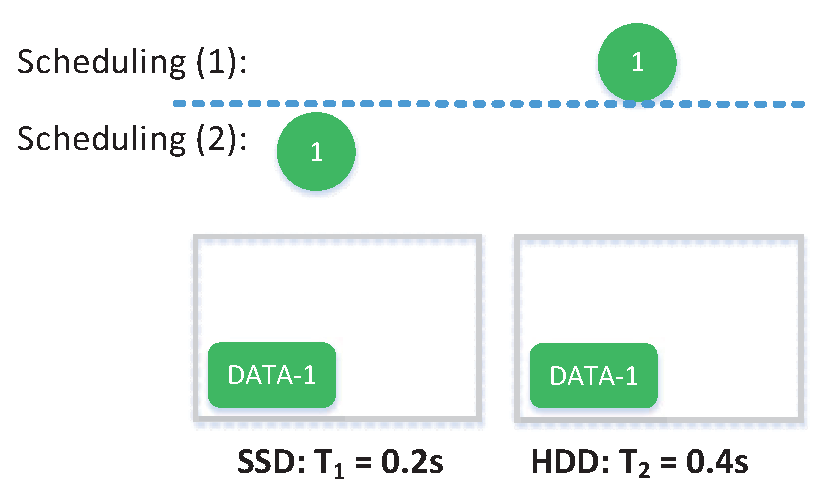
\includegraphics[width=4.78cm]{fig_example1_4.eps}
        \centerline{\footnotesize{(1) = $max$\{0, $0.4s$\},}}\\
        \centerline{\footnotesize{(2) = $max$\{$0.2s$, 0\}.}}\\
         \centerline{(a) Type of storage.}\\
    \end{minipage}
    \begin{minipage}{3.95cm}
        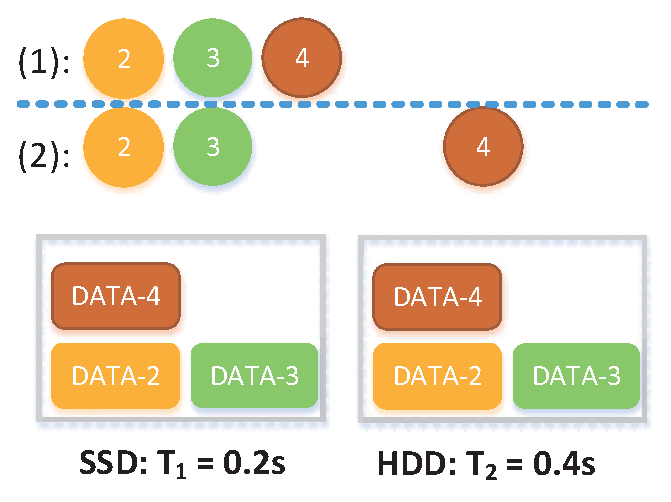
\includegraphics[width=3.95cm]{fig_example2_3.eps}
        \centerline{\footnotesize{(1) = $max$\{$0.2s*3$, 0\},}}\\
        \centerline{\footnotesize{(2) = $max$\{$0.2s*2$, 0.4s\}.}}\\
         \centerline{(b) Load of storage.}\\
    \end{minipage}
    \vspace{-0.4cm}
    \caption{Two aspects that affect the task reading time: (a) type of storage, (b) Load of storage. Delicate method, i.e., Scheduling 2, improves 50\%, 33\% over scheduling 1, respectively.}
    \label{Fig:example}
    \vspace{-0.2cm}
\end{figure}

%denoted by \{$r_l^1$, $r_l^2$,... $r_l^{C}$\}
\subsection{System Model}

The major notations used are shown in table \ref{table-notations}. The data center is equipped with heterogeneous disks, and we denote by $\mathcal{D}$ the heterogeneous disks set, $\mathcal{D}$ = \{1, 2, ...,$|\mathcal{D}|$\}. Each disk-i corresponds to a different reading time for one task, denoted by $T_i$, $i \in \mathcal{D}$.
$\mathcal{M}$ is defined as the set of data in data center, $\mathcal{M}$ = \{1, 2, ..., $|\mathcal{M}|$\}. Each data-l has $C$ replicas whose size $\tau$, e.g., 64MB or 128MB,  stored on $C$ different disks. $\pi_l^{i}$ is a binary variable indicating whether data-l is stored in disk-i or not. More concretely, we define $\pi_l^{i}$ as
\begin{equation}
\pi_l^{i} =
\begin{cases}
1, &\text{if the disk-i stores a replica of the data-l,}\\
0, &\text{otherwise,}
\end{cases}\nonumber
\end{equation}

When the job arrives, the job will be divided into parallel tasks, denoted by $\mathcal{T}$ = \{1, 2,  ..., $\mathcal{|T|}$ \}. Each task-j corresponds to one data $\phi_j$, where $\phi_{j}$ represents the data that task-j need to read. Since there are $C$ replicas for each data deployed in $C$ disks, task-j can read $\phi_j$ among the $C$ disks, denoted by \{$d_{1}^j$, $d_{2}^j$,... $d_{C}^j$\}.


$I_i^j$ is a decision variable indicating whether task-j choose to read the replica stored in disk-i or not. Specificly, we define $\pi_l^{i}$ as
\begin{equation}
I_i^j =
\begin{cases}
1, &\text{\tabincell{l}{if the task-j chooses to read the replica \\stored in disk-i,}}\\
0, &\text{otherwise,}
\end{cases}\nonumber
\end{equation}

Then, we denote by $load_i$ the reading time of all tasks for the disk-i, $load_{i}$ = $\sum_{j}I_i^j*T_i$. In order to balance the use of heterogeneous and speed up the reading time of data analytical tasks, our objective is to minimize the maximum disk's $load$.

\begin{table}[!t]
	\Large
	\centering
	\footnotesize
	\renewcommand\arraystretch{1.2}
	\caption{THE MAJOR NOTATIONS USED IN THIS PAPER.}
	\label{table-notations}
	\begin{tabular}{c|l}
		\hline\hline
		Variable & Description\\

		\hline
		$T_{i}$ & \tabincell{l}{The time of reading a replica from disk-i } \\
		\hline
		$\phi_j$ & The index of data that task-j needs, $\phi_j$ $\in$  $\mathcal{M}$ \\
		\hline
		$d_{r}^j$ & \tabincell{l}{The index of disk which stores data $\phi_j$'s r-th replica} \\
		\hline
		$\pi_{l}^{i}$ & \tabincell{l}{A binary variable indicating if data $m_l$ are \\stored at disk-i or not} \\
		\hline
		$\phi_j$ & The data that task-j needs \\
		\hline
		$N_i$ & Number of tasks which reads data from disk-i \\
		\hline
		$\tau$ & Size of each data replica in data center \\
		\hline
		$C$ & The number of replicas for each data. \\
		\hline\hline
		Decision variable & Description\\
		\hline
		${I}_i^j$ & \tabincell{l}{A binary variable indicating if task $t_{i}$ choose \\ to read the replica stored in $d_{i}$ or not}\\
		\hline	
	\end{tabular}
\end{table}

\subsection{Workload-Aware Scheduling problem for Heterogeneous-storage $(\rm{WASH})$} \label{WASH}
%$\mathcal{AP} \mathbb{AP}$ (~/~)
A large number of tasks are running in the cluster of data centers. If the schedulers are unaware of the heterogeneity of disks, it is easily causing the unbalanced use on disks, resulting in elongating the latency  on analytical tasks. To avoid such situation, we propose Workload-Aware Scheduling problem for Heterogeneous-storage (WASH), as shown below. The optimization goal is to minimize the maximum disk load. Finally, by determining the value of the decision variable $I_i^j$, the appropriate disk is selected for each task to read the corresponding data. Detailed description is as follows:
\begin{align}
Min:&\;\;\;\;\;\max\limits_{i}\{\sum_{j}I_i^j*T_i\}\;\;\;\;\;\;[\rm{WASH}]\nonumber\\
s.t. 
&\;\;\;\;\;\sum_{i}I_i^j = 1,\;\;\forall j,\label{task-cons}\\
&\;\;\;\;\;I_i^j \leq \pi_{\phi_j}^{i},\;\;\forall i,j\label{data-cons},\\
&\;\;\;\;\;I_i^j\in\{0,1\},\;\;\forall i,j.\label{def-cons}
\end{align}

Constraint (\ref{task-cons}) guarantees that task-j can only fetch data $\phi_j$ from one source disk. Constraint (\ref{data-cons}) guarantees that task-j can only select from those disks containing its input data. If one replica of data $\phi_j$ is stored in disk-i, then $\pi_{\phi_j}^{i}$ = 1, otherwise $\pi_{\phi_j}^{i}$ = 0. Constraint 3 denotes the domain of decision variables, which can only be 0 or 1. $I_i^j$ = 1 indicates that task-j selects the replica stored on disk-i as input, while $I_i^j$ = 0 is on the contrary.The key to solve WASH problem is to determine the value of decision variables {$I_i^j$}. 

Next, we show the NP-hardness of this problem. WASH problem can be reduced from the integer linear programming (ILP) problem. The ILP problem is NP-hard, and it follows that WASH problem is NP-hard. The specific proof is as follows.

\emph{\textbf{Theorem 1:}} The WASH problem is NP-hard.

\emph{Proof:} See Appendix.


\section{DESIGN of ALGORITHMS FOR WASH PROBLEM}\label{DESIGN_ALGORITHM}

Our aim is to find the optimal assignment of each reading task among the heterogeneous disks. However, due to the hardness of WASH problem, the optimal assignment can not be obtained in polynomial time. In order to solve WASH, we first design a heuristic algorithm based on greedy idea, named WASH-greedy. However, extensive experiments shows that WASH-greedy has a little improvement over the baseline, i.e., Hadoop-default which is storage-unaware. Furthermore, In order to solve WASH better, we design a randomized algorithm (WASH-rdm) which chooses source devices based on delicate calculated probabilities and can be proved concentrated on its optimum with high probability, i.e., 1- O($e^{-t^2}$), through our theoretical analysis.

\subsection{Heuristic Alogrithm}\label{Heuristic}

In this subsection, we first introduce our heuristic algorithm, WASH-greedy, specificly. Based on a greedy idea, while finding the assignment for each task, the disk which has the minimum reading time of one replica, i.e. $T_i$, will be selected by WASH-greedy. Note that the selected disk must store the replica that the task need. Then, the scheduler will use the assignments to schedule each reading task. To be more specific, WASH-greedy is as follows:

%Alogoritm1
\begin{algorithm}

	\textbf{Require:} Find an assignment of each reading task-j, $j \in \mathcal{T}$, among the disks which store one replica of data $\phi_j$.

	\begin{algorithmic}[1]
		
		\State $Result$ $\gets$ \{\}\label{WASH-greedy:init}
		\For{each task-j, ($j \in \mathcal{T}$)} 
			\State \{$d_{1}^j$, $d_{2}^j$,... $d_{C}^j$\} = $f(\phi_j)$
		
		$//$Function $f$ is a mapping from data to disks which stores the replicas of the data.
			\State $d_{j_{min}}$ $\gets$ $\min\limits_{d \in \{d_{1}^j, d_{2}^j,... d_{C}^j\} }$\{$T_{d_{j_l}}$\}
		
			\State $Result$ $\gets$ $Result$ $\cup$
			\{$\left \langle j, d_{j_{min}}\right \rangle$\}
		\EndFor
	
	\State Use $Result$ to schedule each task-j, $j \in \mathcal{T}$.
	\end{algorithmic}
	\caption{WASH-greedy}\label{WASH-greedy}
\end{algorithm}

Algorithm \ref{WASH-greedy:init} shows the detailed of WASH-greedy. Line 1-4 initializes $Result$ = \{\}. Line 2-6 is to select a source disk for each task-j. In line 3, function $f$ is used for task-j to find all disks that store replicas of data $\phi_j$, denoted by \{$d_{1}^j$, $d_{2}^j$,... $d_{C}^j$\}. Next, in line 4, the disk with minimum reading time is selected from the $C$ disks. After putting the task-j and disk $d_{j_l}$ into the set $Result$, the algorithm completes one assignment of a task. After $\mathcal{|T|}$ iterations, WASH-greedy come to an end.

%Next, an example is given to illustrate the algorithm. In datacenter, there exits a set of heterogeneous disks $\mathcal{D}$= \{$d_1$, $d_2$, $d_3$, $d_4$\} with $T_i$ $T_1$ = 0.3,  $T_2$ = 0.1,  $T_3$ =0.2 and $T_4$ =0.2, respectively. Data set $\mathbb{M}$ = \{$m_1$, $m_2$, $m_3$, $m_4$\} are stored as Fig.\ref{fig1}. Obviously, each data has two replicas. When query tasks $\mathcal{T}$= \{$t_1$, $t_2$, $t_3$, $t_4$\} ($\phi_j$ = j, 1$\leq$j$ \leq$4) comes, the algorithm WASH-greedy runs as follows: %($\phi_j$ = j (1 $\leq$j$ \leq$ 4, task $t_j$'s input is $m_j$ which equals the DATA-j in Fig.\ref{fig1}))

Next, we use an example to illustrate WAHS-greedy. In data center, there exits a set of heterogeneous disks $\mathcal{D}$= \{1, 2, 3, 4\} with $T_1$ = 0.2,  $T_2$ = 0.25,  $T_3$ =0.4 and $T_4$ =0.6, respectively. Data set $\mathcal{M}$ = \{1, 2, 3, 4\} are stored as Fig.\ref{fig1}. Obviously, each data has two replicas. When query tasks $\mathcal{T}$= \{1, 2, 3, 4\} ($\phi_j$ = j, 1$\leq$j$ \leq$4) comes, the algorithm WASH-greedy runs as follows: %($\phi_j$ = j (1 $\leq$j$ \leq$ 4, task $t_j$'s input is $m_j$ which equals the DATA-j in Fig.\ref{fig1}))

Initial: Reslut = \{\}
\begin{itemize}
	\item \textbf{Round 1}:for task-1:
	 f($\phi_1$) = \{1, 2\} = \{DISK1, DISK2\}\\
	 $1$ = $\min$\{$T_1$ = 0.2, $T_2$ = 0.25\}\\
	Result = Result $\cup$ $\left \langle 1, 1\right \rangle$ = \{$\left \langle 1, 1\right \rangle$\}
	\item \textbf{Round 2}:for task-2:
	f($\phi_2$) = \{2, 3\}\\
	$2$ = $\min$\{$T_2$ = 0.25, $T_3$ = 0.4\}\\
	Result = Result $\cup$ $\left \langle 2, 2\right \rangle$ = \{$\left \langle 1, 1\right \rangle$, $\left \langle 2, 2\right \rangle$\}
	\item \textbf{Round 3}:for task-3:
	f($\phi_3$) = \{3, 4\}\\
	$3$ = $\min$\{$T_3$ = 0.4, $T_4$ = 0.6\}\\
	Result = Result $\cup$ $\left \langle 3, 3\right \rangle$ = \{$\left \langle 1, 1\right \rangle$, $\left \langle 2, 2\right \rangle$,  $\left \langle 3, 3\right \rangle$\}
	\item \textbf{Round 4}:for task  $4$:
	f($\phi_4$) = \{1, 4\}\\
	$1$ = $\min$\{$T_1$ = 0.2, $T_4$ = 0.6\}\\
	Result = Result $\cup$ $\left \langle 4, 1\right \rangle$ = \{$\left \langle 1, 1\right \rangle$, $\left \langle 2, 2\right \rangle$,  $\left \langle 3, 3\right \rangle$, $\left \langle 4, 1\right \rangle$\}	
	\item \textbf{Round 5}:for task-5:
	f($\phi(5)$) = \{2, 4\}\\
	$2$ = $\min$\{$T_2$ = 0.25, $T_4$ = 0.6\}\\
	Result = Result $\cup$ $\left \langle 5, 2\right \rangle$ = \{$\left \langle 1, 1\right \rangle$, $\left \langle 2, 2\right \rangle$,  $\left \langle 3, 3\right \rangle$, $\left \langle 4, 1\right \rangle$, $\left \langle 5, 2\right \rangle$\}	
	
\end{itemize}
\begin{figure}[!t]
	\centering
	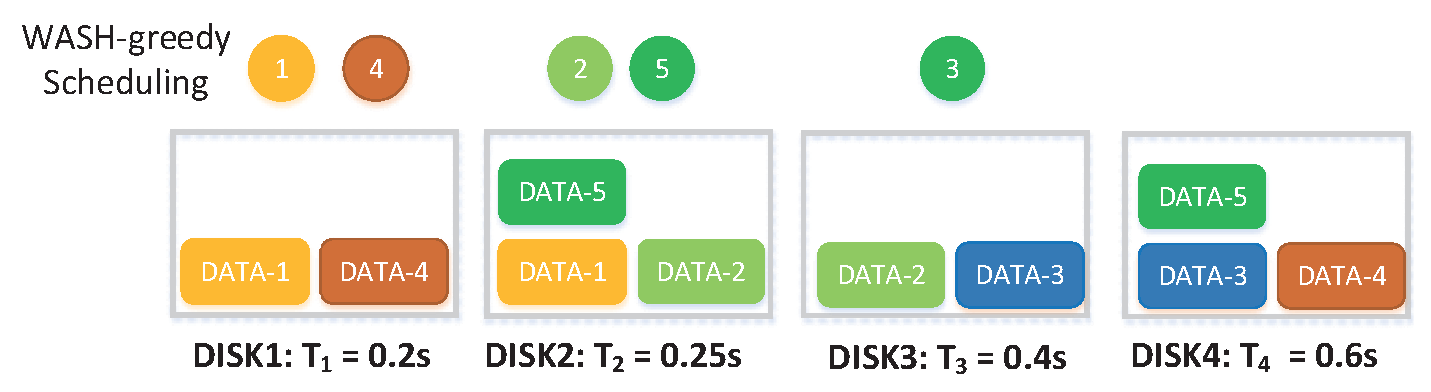
\includegraphics[height=0.8in]{fig1_9.eps}
	\caption{An execution example of greedy algorithm  }
	\label{fig1}
\end{figure}
\begin{figure}[!t]
	\centering
	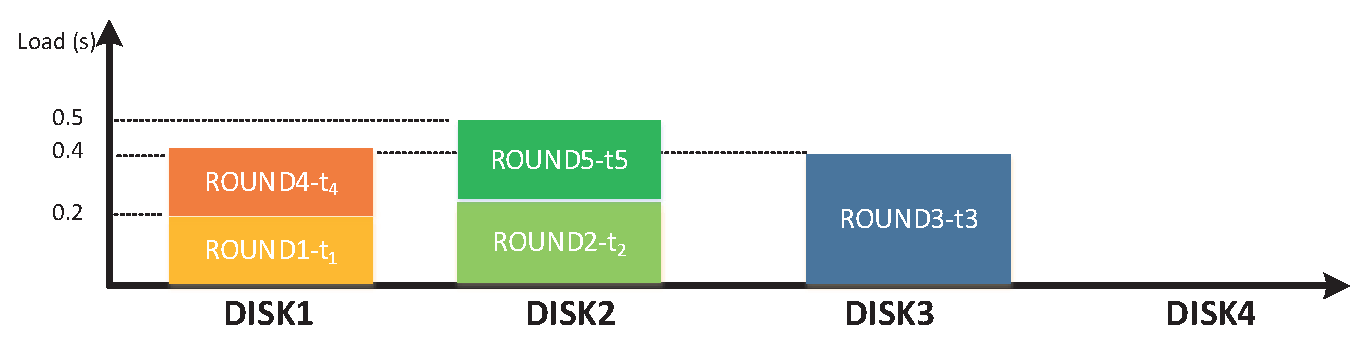
\includegraphics[height=0.8in]{fig2_2.eps}
	\caption{The process of WASH-greedy algorithm execution for the data stored as Fig.\ref{fig1}. }
	\label{fig2}
\end{figure}

Then, the four tasks read data following the assignment of \{$\left \langle 1, 3\right \rangle$, $\left \langle 2, 1\right \rangle$,  $\left \langle 3, 2\right \rangle$, $\left \langle 4, 1\right \rangle$, $\left \langle 5, 2\right \rangle$, $\left \langle 6, 1\right \rangle$\} to read data.The specific steps of WASH-greedy algorithm is shown in Fig.\ref{fig2}.

\subsection{Randomized Alogrithm}\label{Randomized}

In the previous subsection \ref{Heuristic}, we design a greedy heuristic algorithm to solve WASH. However, our extensive experiments prove low-performance of WASH-greedy. Therefore, in this subsection, we design a randomized algorithm, named WASH-rdm, which chooses source devices based on delicate calculated probabilities. Specificly, by relaxing the WASH problem to WASH-relaxation problem, then our algorithm uses linear programming tools to solve WASH-relaxation. The decomposition obtained by linear programming is a fraction rather than an integer, which represents the preference when selecting source disks. Subsequently, we prove WASH-rdm is concentrated on its optimum with high probability, i.e., 1- O($e^{-t^2}$), through our theoretical analysis where $t$ is the concentration bound.

\paragraph{\textbf{Relaxation of WASH Problem}} According to the previous analysis \ref{WASH}, this problem is NP-hard, whose optimal assignment of each task cannot be obtained in polynomial time. But linear programming (LP) problem is solvable in polynomial time, a natural point of view is to relax the WASH problem to LP. The method is to change the domain of decision variables from integer domain \{0, 1\} to real domain [0, 1], i.e., WASH-relaxation. Such process is named \textbf{relaxation}. The solution of WASH-relaxation provides a lower bound for the original WASH problem (WASH is a minimization problem. For the maximization problem is on the contrary). Next, based on the solution of linear programming, the fractional solution is mapped back to integer in some way, which is named \textbf{rounding}. 
 \begin{align}
 Min:&\;\;\;\;\;\max\limits_{i}\{\sum_{j}p_i^j*T_i\}\;\;\;\;\;\;[\rm{WASH-relaxtion}]\nonumber\\
 s.t. 
 &\;\;\;\;\;\sum_{i}p_i^j = 1,\;\;\forall j,\nonumber\\
 &\;\;\;\;\;p_i^j \leq \pi_{\phi_j}^{i},\;\;\forall i,j,\nonumber\\
 &\;\;\;\;\;p_i^j \in[0, 1],\;\;\forall i,j.\nonumber
 \end{align}

 Based on relaxation-rounding, we propose WASH-rdm algorithm. More concretely, WASH-rdm is described as follows: 

  \begin{algorithm}
 	%\renewcommand{\thealgorithm}{}
 	\textbf{Require:} Find an assignment of each reading task-j, $j \in \mathcal{T}$, among the disks which store one replica of data $\phi_j$. %and $d_i$ stores data $\phi_j$.
 	\begin{algorithmic}[1]	
 		\State $Result$ $\gets$ \{\}
 		\State \{$p_i^j$\} = WASH-relaxation		
 		
 		$//$ \{$p_i^j$\} is the solution of WASH-relaxation problem. 
 		
 		\State According to \{$p_i^j$\}, use rounding strategy and get \{$I_i^j$\}
 		\For{$\forall$ $i$, $j$, ($i \in \mathcal{D}$, $j \in \mathcal{T}$) } 
 			\If{$I_i^j$ == 1}
 			\State $Result$ $\gets$ $Result$ $\cup$ 	
 			\{$\left \langle j, i\right \rangle$\}
 			\EndIf
 		\EndFor	
 		\State Use $Result$ to schedule each task-j, $j \in \mathcal{T}$.
 	\end{algorithmic}
 	\caption{WASH-rdm}\label{WASH-rdm}
 \end{algorithm}

 The detailed of WASH-rdm is shown in Algorithm \ref{WASH-rdm}. Line 1 initializes the set of $Result$, which stores the final results. In the second line, WASH-relaxation problem is solved by linear programming tools. The third line uses rounding strategy to convert fractional solution to integer solution. Line 4-9 organize the results. Then the tasks will read the disk according to $Result$. The specific rounding strategies are as follows:
 
 The value of \{$p_i^j$\}  $\in$ [0, 1] which shows the correlation between task-j and disk-i. Then, we can select a disk-i for task-j with probability \{$p_i^j$\}. The method is to use the parameter $q_j$, which is randomly selected in (0,1]. If the $q_j$ $\in$ ($\sum p_{r-1}^{j}$, $\sum p_{r}^{j}$], then $I_r^j = 1$, otherwise, $I_i^j$ = 0 ($\forall$ $i$, $i \ne r$). This approach ensures only one disk can be selected for each task.%For each task $t_j$, the corresponding decision variables are \{$p_0^j$,$p_i^j$, ..., $p_i^j$\}. 


\paragraph{\textbf{Analysis of WASH-rdm Algorithm}}

In this section, we will prove that our WASH-rdm can be proved concentrated on its optimum with high probability, i.e., 1- O($e^{-t^2}$). Firstly, we prove that the difference between reading time of disk-i contributed by any task-j and expectation is martingales sequence \cite{b12}. Secondly, Based on the martingales sequence, we use Azuma's Inequality to illustrate the bound between the feasible solution and the optimal solution.
\begin{figure*}[!t]
	\centering
	\subfigure[Small Workload ]{\label{Fig:instance1}\includegraphics[height=1.6in]{fig_instance1_4.eps}}\quad\quad %quad 表示图像的间距
	\subfigure[Medium Workload ]{\label{Fig:instance2}\includegraphics[height=1.6in]{fig_instance2_4.eps}}\quad\quad
	\subfigure[Large Workload
	]{\label{Fig:instance3}\includegraphics[height=1.6in]{fig_instance3_4.eps}}
	\vspace{-1ex}
	\caption{Comparison of WASH-rdm and other Algorithm on different Workloads. \ref{Fig:instance1} denotes the results on Small Workload which has about 500 tasks. \ref{Fig:instance2} denotes the results on Medium Workload which has about 2000 tasks.
	\ref{Fig:instance3} denotes the results on Large Workload which has 5000 tasks. X-axis denotes the disk. Y-axis denotes the load of each disk after running the three algorithms.}
	\label{Fig:instance}
	\vspace{-1ex}
\end{figure*}

\emph{\textbf{Theorem 2:}} $Pr[SOL(\text{WASH-rdm}) - OPT(\text{WASH}) \leq t] \geq 1 - O(e^{-t^2})$.

\emph{\textbf{Proof:}}

$SOL(\text{WASH-rdm})$ denotes the feasible solution found by WASH-rdm  and $OPT(\text{WASH})$ denotes the optimum solution of WASH problem.

Firstly, task-j's contribution to disk-i's load is expressed as:
 \begin{align}
&\;\;\;\;\;Z_i^j = I_i^j*T_i
\end{align}
From the rounding strategy in Algorithm \ref{WASH-rdm}, we can get that:
 \begin{align}
&\;\;\;\;\;Pr[I_i^j = 1] = p_i^j,\;\;\forall i,j \nonumber
\end{align}
%Therefore

The expectation of $Z_i^j$ is
\begin{align}
E[Z_i^j] &\;\;\;= E[I_i^j]*T_i \nonumber\\
&\;\;\;= (Pr[I_i^j = 1] * 1 + Pr[I_i^j = 0] * 0)*T_i \nonumber\\
&\;\;\;= p_i^j*T_i\label{prove:expect}
\end{align}

The difference between $Z_i^j$ and $E[Z_i^j]$ defines as
\begin{align}
Q_i^j = Z_i^j - E[Z_i^j]\label{prove:diff}
\end{align}

For the all $\mathbb{|T|}$ tasks, $L_i^{\mathbb{|T|}}$ denotes the sum of $Q_i^j$ in disk $i$:
\begin{align}
L_i^{\mathbb{|T|}} = \sum_{j = 1}^{\mathbb{|T|}} Q_i^j
= \sum_{j = 1}^{\mathbb{|T|} - 1} L_i^j + Q_i^{\mathbb{|T|}} \label{prove:L_margin}
\end{align}
Then, on the condition $L_i^{1}$, $L_i^{2}$, ..., $L_i^{r-1}$, the expectation of $L_i^{r}$ is:
\begin{align}
&E[L_i^{r}|L_i^{1}, L_i^{2}, ..., L_i^{r-1}] \nonumber\\
&\overset{\text{(\ref{prove:L_margin})}}{=}E[L_i^{r-1} + Q_i^{r} |L_i^{1}, L_i^{2}, ..., L_i^{r-1}] \nonumber\\
&\overset{\text{}}{=}E[L_i^{r-1} |L_i^{1}, L_i^{2}, ..., L_i^{r-1}]
+ E[Q_i^{r} |L_i^{1}, L_i^{2}, ..., L_i^{r-1}] \nonumber\\
&\overset{\text{(\ref{prove:diff})}}{=}L_i^{r-1} + E[Z_i^r - E[Z_i^r] |L_i^{1}, L_i^{2}, ..., L_i^{r-1}]\nonumber\\
&=L_i^{r-1} + E[Z_i^r|L_i^{1}, L_i^{2}, ..., L_i^{r-1}]
-E[E[Z_i^r] |L_i^{1}, L_i^{2}, ..., L_i^{r-1}]\nonumber\\
&=L_i^{r-1} + E[Z_i^r] - E[Z_i^r]\nonumber\\
&=L_i^{r-1}\label{prove:marginsq}
\end{align}
Therefore, $L_i^{1}$, $L_i^{2}$, ..., $L_i^{|\mathcal{T}|}$ are martingales sequence \cite{b13}. For completeness, we let $L_i^{0}$ = 0. And $\forall r \geq 1$, we have:
\begin{align}
  |L_i^r - L_i^{r-1}|\overset{\text{(9a)}}{=} |Q_i^{r}| \overset{\text{(9b)}}{=} |Z_i^j - E[Z_i^j]|\leq g_i^r\label{prove:bound1}\\
  g_i^r = \max\{T_i -  E[Z_i^j], E[Z_i^j]\}\label{prove:bound}
\end{align}

In (\ref{prove:bound1}), the existences of (9a) and (9b) are due to \ref{prove:L_margin} and \ref{prove:diff}, respectively. From above (\ref{prove:bound}), any two adjacent values, i.e., $L_i^r$, $L_i^{r-1}$, in the martingales sequence have constant bounds $g_i^r$. Based on (\ref{prove:marginsq}) and (\ref{prove:bound}), we can use Azuma's Inequality. Then, 
\begin{align}
Pr\{L_i^{|\mathcal{T}|} - L_i^{0} \geq t\} \leq exp\{-\frac{t^2}{2\sum_{ i = 1 }^{|\mathcal{T}|}(g_i^k)^2}\} \label{prove:azuma}
\end{align}

Substitute equations (\ref{prove:diff}) and (\ref{prove:L_margin}) into the upper equation (\ref{prove:azuma}). Then, 
\begin{align}
Pr\{\sum_{j = 1}^{|\mathcal{T}|} Z_i^j - 
	\sum_{j = 1}^{|\mathcal{T}|} E[Z_i^j]\geq t\} \leq exp\{-\frac{t^2}{2\sum_{ i = 1 }^{|\mathcal{T}|}(g_i^k)^2}\} \label{prove:azuma1}
\end{align}
 The (\ref{prove:azuma1}) is equal to:
\begin{align}
Pr\{\sum_{j = 1}^{|\mathcal{T}|} Z_i^j \leq \sum_{j = 1}^{|\mathcal{T}|} E[Z_i^j] + t\} & \geq 1 - exp\{-\frac{t^2}{2\sum_{ i = 1 }^{|\mathcal{T}|}(g_i^k)^2}\}\nonumber\\
& = 1 - O(e^{-t^2})\label{prove:azuma3}
\end{align}

Let $S_i$  = $\sum_{j = 1}^{|\mathcal{T}|} Z_i^j$,
$E_i$ = $\sum_{j = 1}^{|\mathcal{T}|} E[Z_i^j]$
$\overset{\text{(a)}}{=}$
$\sum_{j = 1}^{|\mathcal{T}|} p_i^j*T_i$, where the existence of (a) is due to \ref{prove:expect}. Then,
\begin{align}
Pr\{S_i \leq U_i + t\} \geq 1- O(e^{-t^2}) \label{prove:SU}
\end{align}

$S_i$ represents the load of disk-i which is the result of ILP. And $E_i$ denotes the expectation which is the result of LP. Because LP provides a lower bound for the optimal solution of ILP problem (WASH is a minimization problem. For the maximization problem is on the contrary), we have:
\begin{align}
E_i \leq OPT(\text{WASH})\label{prove:OPT}
\end{align}

Take $S_u$, $E_v$ as
\begin{align}
	S_u = S_{max} = \max_i S_i\\
	E_v = E_{max} = \max_i E_i\label{prove:Emax}
\end{align}

Then, we have the following inequalities,
\begin{align}
SOL(\text{WASH-rdm}) = S_u  
\overset{\text{(18a)}}{\leq}  E_u+t
\overset{\text{(18b)}}{\leq} E_v+t\nonumber\\
\overset{\text{(18c)}}{\leq} OPT(\text{WASH})+t\label{prove:SOL-OPT}
\end{align}

In (\ref{prove:SOL-OPT}), the existences of (18a), (18b) and (18c) are due to (\ref{prove:azuma3}), (\ref{prove:Emax}) and (\ref{prove:OPT}), respectively.  From (\ref{prove:SU}) and (\ref{prove:SOL-OPT}), we can conclude that,
\begin{align}
Pr\{SOL(\text{WASH-rdm})<OPT (\text{WASH})+t\}\nonumber\\ 
\geq 1 - O(e^{-t^2})\label{prove:result}
\end{align}

Observed from the (\ref{prove:result}), the feasible solution $SOL(\text{WASH-rdm})$ found by the algorithm and the optimal solution OPT (WASH) are approximated by probability $1 - O(e^{-t^2})$. When hundreds of tasks are deployed with $1 - O(e^{-t^2})$ = 0.85, the value of $t$ is acceptable, only a few millisecond.\hfill $\qedsymbol$

\section{PERFORMANCE EVALUATION}\label{PERFORMANCE_EVALUATION}

In this section, we make extensive simulations, comparing our algorithm, i.e., WASH-rdm, with WASH-rdm and storage-unaware scheduling algorithm. The results of simulations show that performance of our proposed WASH-rdm can improves by up to 55\% and 25\%, respectively.
\subsection{Simulation Settings}\label{SCM}
Usually, the traditional scheduling mechanism are not aware of the types and workloads of the disks. Such as Hadoop, the scheduler selects source device that stores the related replica of tasks in random strategy, which we call Hadoop-default. In our extensive simulation, we compare our WASH-rdm with WASH-greedy and Hadoop-default.

\textbf{Workload:} Referring to the characteristics of Google traces \cite{b20}, we classify workload into three categories: Small Workload, Medium Workload and Large Workload, as shown in TABLE \ref{tab:workload}. In Small Workload, most of the jobs have 1-150 tasks. In has Large Workload, there are 50\% of the jobs that has over 50 tasks. The Medium Workload is in the middle of them.

\begin{table}[htbp]
	\caption{THE DIFFERENT TRACES USED FOR EXPERIMENT}
	\begin{center}
		\begin{tabular}{|c|c|c|c|}
			\hline
			 \diagbox{Traces}{Number of tasks} & 1-150 & 150-500 & $\ge$ 500\\
			\hline
			Small Workload & 96\% & 2\% & 2\%\\
			\hline
			Medium Workload & 50\% & 40\% & 10\%\\
			\hline
			Large Workload & 40\% & 10\% & 50\%\\
			\hline
		\end{tabular}
		\label{tab:workload}
	\end{center}
\end{table}

\textbf{Setting:}
In distributed file systems \cite{b19}, data is distributed uniformly on disk. Therefore, in this experimental environment, we uniformly deploy 200000 data with three data replicas by default, each data block size $\tau$ = 128MB. 500 disks are set up by default. The $T_i$ of the disk in the cluster is between 10ms and 500ms. 
\begin{figure*}[!t]
	\centering
	\subfigure[Results under varilous setting on Workloads ]{\label{Fig:completeWorkload}\includegraphics[height=1.6in]{figcomplete1_5.eps}}\quad\quad %quad 表示图像的间距
	\subfigure[Results under different Heterogeneity cluter. ]{\label{Fig:completeHeter}\includegraphics[height=1.6in]{figcomplete2_5.eps}}\quad\quad
	\subfigure[Results under varilous setting on reolicas number
	]{\label{Fig:completeRep}\includegraphics[height=1.6in]{figcomplete3_5.eps}}
	\vspace{-1ex}
	\caption{Comparison of WASH-rdm and other Algorithm on different workloads, different heterogenelity cluter and different replica number $C$. \ref{Fig:completeWorkload} denotes effect of different workloads on reading time. \ref{Fig:completeHeter} denotes the reading time of the three algorithm on different Heterogeneity cluter. \ref{Fig:completeRep} denotes the reading time of the three algorithm when $C$ is different. Y-axis denotes the reading time of all tasks which has been normalized.}
	\label{Fig:complete}
	\vspace{-3ex}
\end{figure*}

\subsection{Simulation Results}

For convenience of display, Fig.\ref{Fig:instance}. shows the results under different workloads upon 50 disks. X-axis denotes the disks. Y-axis denotes the load of each disk after running the three algorithms. The lower the peak of the curve, the better the result. The black dotted line represents the execution result of Algorithm WASH-greedy, and the green line represents the execution result of Algorithm WASH-rdm. Overall, we can see that our algorithm performs better than Hadoop-default. As shown in Fig.\ref{Fig:instance1}, in the small workload, the result of Hadoop-default has large fluctuations. This is a result of that hadoop-default is not aware of the $T_i$ and load of the disk when selecting a replica for the task. Even if the tasks are deployed uniformly on disks, the disk with low performance may have a relatively large load. In Fig. \ref{Fig:instance1}, low performance disks will have high peaks. Completion of all parallel tasks is the end of the big data processing job. Therefore, the task reading data from the disk with poor performance will be the bottleneck of data processing job. For example, Hadoop-default causes the tasks of reading data from disk-2 to be the bottleneck of big data processing in the Fig.\ref{Fig:instance1} which is 654. Algorithms WASH-greedy and WASH-rdm can maintain roughly all disks at a lower load, less than 300. The reason is that WASH-greedy can select the disk to read for the task according to load of the disks and WASH-rdm can select the disk to read for the task according to load of the disks the performance of the disk. The maximum load of WASH-greedy algorithm is 261 in disk-12. Compared with the Hadoop-default, the performance is improved by 64\%. The maximum load of WASH-rdm algorithm is disk-4, and the corresponding load is 284. Compared with the baseline algorithm, the performance of WASH-rdm algorithm improves 57\%.
As the number of tasks increases, the load on all disks increases. For example, in Fig.\ref{Fig:instance2}, when the number of tasks is about 2000, in Hadoop-default algorithm the maximum load is 2009 in disk-9. The results of WASH-greedy and WASH-rdm are that 784 in disk-8  and 770 in disk-6, respectively. The performance of our algorithm improves by 61\% and 62\%. 
When the number of tasks becomes larger, in the large Workloads of Fig. \ref{Fig:instance3}, the maximum load obtained by the three algorithms are 5546,2205 and 2646. WASH-greedy increases by 60\% and WASH-rdm performance improves by 52\%.
 
Next, we study the impact of different factors workloads, degree of heterogeneity and the number of data replicas, on the load upon the default configuration. In Fig.\ref{Fig:completeWorkload}, the horizontal X-axis represents different workloads, and the Y-axis represents the maximum load in the cluster, which has been normalized. In the previous part, impact of Workloads is that the overall load on disk shows an increasing trend as the Workloads gets larger. Fig.\ref{Fig:completeWorkload} shows the difference among the three workloads. The performance of our proposed algorithm can always be improved by 60\% on average. Next, we observed the effect of degree of heterogeneity on the load. We divide the heterogeneity of the cluster into two kinds. One is that the $T_i$ of disks is evenly distributed between 10ms and 100ms, named Low Heterogeneous Cluster. Another is High Heterogeneous Cluster, where the $T_i$ of disks are evenly distributed between 10ms and 500ms. Other conditions are configured by default. From Fig.\ref{Fig:completeHeter}, when the degree of heterogeneity gets larger, the overall load shows an increasing trend. This is because the large the degree of heterogeneity, the greater the performance difference between disks. This leads to hard balancing of disk loads. Through \ref{Fig:completeHeter}, we find that our algorithm can also improve the performance of 40-50\% in clusters with high heterogeneity. Finally, we analyze the impact of the amount of data replicas on disk load. We set the number of data replicas as 2, 3 and 5. Observe that the higher the number of replicas, the lower the disk load. Reason for it is that with the number of data replicas increasing, the probability of data being deployed on high performance disks increases. Selecting data on high-performance disks at this time will greatly accelerate the completion of tasks. When $C$ = 5, our algorithm can achieve 65\% performance improvement.
 
 All in all,  the performance of the two algorithms proposed by us has reached an average of 55\% improvement over baseline algorithm on average under different conditions.



\section{CONCLUSION}\label{CONCLUSION}
In this paper, in order to keep the balanced use on disks and speed up the reading time of data analytical tasks, the type of heterogeneous-storage and the workloads of storage devices both should be taken into consideration. Therefore, we formulate the workload-aware scheduling problem for heterogeneous-storage, showing its NP-hardness and design a randomized algorithm with performance-guarantee. The results of our simulation show that our proposed WASH-rdm speeds up data analytics up to 55\% over the baseline algorithms.
%\section*{Acknowledgment}
%None

\section*{APPENDIX}

\textbf{\normalsize{The Proof of Theorem 1}}
\vspace{1ex}

The canonical form \cite{b11} of ILP is described below.

For $m\times n$ matrix \textbf{A}
\begin{align}
Min:&\;\;\;\;\;\textbf{c}^T\textbf{x}\;\;\;\;\;\;[\rm{ILP}]\label{ILP}\\
s.t. 
&\;\;\;\;\;\textbf{A}\textbf{x}\geq \textbf{b},\nonumber\\
&\;\;\;\;\;\textbf{x} \geq0\;and\;\textbf{x} \in \mathbb{Z}^n.\nonumber
\end{align}
Taking the special case of WASH problem, the parameters are set as follows:
\begin{itemize}
	\item $\mathcal{D}$ = \{$0$, $1$, $2$\};$T_0$ = 1, $T_1$ = 1, $T_2$=1; $\mathbb{M}$ = \{$m_0$, $m_1$, ..., $m_{n-1}$\}; $C$ = 3
	\item $T$ = \{$0$, $1$, ..., $t_{n-1}$\}
\end{itemize}

It means that there are 3 disks, $0$, $1$, $2$, in the data center, each disk with a $T_i$ of 1. A total of n data, and each data has three replicas which deployed in the three disks, respectively. When the query job arrives, the job is divided into n tasks, \{$t0$, $1$, ..., $n$\} to read n data, \{$0$, $1$, ..., $n$\}, respectively.

For this particular case, the problem description can be modified to:
\begin{align}
Min:&\;\;\;\;\;\max\{\sum_{j}I_0^j, \sum_{j}I_1^j, \sum_{j}I_2^j\}\;\;\;\;\;[\rm{WASH-sp}]\\
s.t. 
&\;\;\;\;\;I_0^j + I_1^j +I_2^j= 1,\;\;\forall j,\nonumber\\
&\;\;\;\;\;I_0^j, I_1^j, I_2^j\in\{0,1\},\;\;\forall j \in[0,n).\nonumber
\end{align}

Let  $x$ = $\sum_{j}I_0^j$, $y$ = $\sum_{j}I_1^j$, $z$ = $\sum_{j}I_2^j$, and the problem description can be modified to:
\begin{align}
Min:&\;\;\;\;\;\max\{x,y,z\}\;\;\;\;\;\;[\rm{WASH-sp}]\\
s.t. 
&\;\;\;\;\;x + y + z = n,\;\label{enlarge-cons}\\
&\;\;\;\;\;0 \leq x, y, z \leq n  \;\;x, y, z\in\mathbb{Z}.\nonumber
%&\;\;\;\;\;0 \leq y \leq n, y\in\mathbb{Z}\nonumber\\
%&\;\;\;\;\;0 \leq z \leq n, z\in\mathbb{Z}\nonumber
\end{align}
In the minimization problem, x + y + z = n can be modified to x + y + z = n and let $R$ denotes $\max\{x,y,z\}$. 

Finally, WASH-sp problem is converted to:
\begin{align}
Min:&\;\;\;\;\;0*x+0*y+0*z+R\;\;\;\;\;\;\;[\rm{WASH-ILP}]\label{WASH-ILP}\\
s.t. 
&\;\;\;\;\;x + y + z \geq n,\;\nonumber\\
&\;\;\;\;\;-x + R \geq 0, \nonumber\\
&\;\;\;\;\;-y + R \geq 0, \nonumber\\
&\;\;\;\;\;-z + R \geq 0, \nonumber\\
&\;\;\;\;\;0 \leq x, y, z \leq n  \;\;x, y, z\in\mathbb{Z},\nonumber\\
%&\;\;\;\;\;0 \leq x \leq n, x\in\mathbb{Z}\nonumber\\
%&\;\;\;\;\;0 \leq y \leq n, y\in\mathbb{Z}\nonumber\\
%&\;\;\;\;\;0 \leq z \leq n, z\in\mathbb{Z}\nonumber\\
&\;\;\;\;\;R \geq 0, R\in\mathbb{Z}.\nonumber
\end{align}

Obviously, WASH-ILP in (\ref{WASH-ILP}) is an instance of ILP in (\ref{ILP}). The decision version of 0-1 ILP (A variation in which only the restrictions must be satisfied, without optimization) is one of Karp's 21 NP-complete problems  \cite{b9}, so ILP is NP-hard. Further, the WASH-ILP problem is NP-hard.

On the one hand, when the optimal solution of WASH-ILP problem is obtained, the corresponding {x, y, z} can be converted into variable {$I_i^j$} in polynomial time by setting the value in \{$I_0^0$, $I_0^1$, ...,$I_0^{x-1}$, $I_1^{x}$, $I_1^{x+1}$, ..., $I_1^{x+y-1}$, $I_2^{x+y}$, $I_1^{x+y+1}$, ..., $I_2^{x+y+z-1}$\} to be 1, which will make the corresponding WASH-sp problem obtain the optimal solution. On the other hand, when the variable \{$I_i^j$\} make the WASH-sp problem obtain the optimal solution, the WASH-ILP also obtains the optimal solution by setting $x$ = $\sum_{j}I_0^j$, $y$ = $\sum_{j}I_1^j$, $z$ = $\sum_{j}I_2^j$. It can be seen from the above that any solution can be polynomially transformed between the WASH-sp and WASH-ILP. Therefore, WASH-sp is NP-hard. 

As a result of that WASH-sp is a special case in WASH, WASH problem is NP-hard.\hfill $\qedsymbol$


\begin{thebibliography}{00}
\bibitem{b1} Ahmad F, Chakradhar S T, Raghunathan A, et al. Tarazu: optimizing mapreduce on heterogeneous clusters[C]//ACM SIGARCH Computer Architecture News. ACM, 2012, 40(1): 61-74.
\bibitem{b2} Zaharia M, Borthakur D, Sen Sarma J, et al. Delay scheduling: a simple technique for achieving locality and fairness in cluster scheduling[C]//Proceedings of the 5th European conference on Computer systems. ACM, 2010: 265-278.
\bibitem{b3} Ananthanarayanan G, Agarwal S, Kandula S, et al. Scarlett: coping with skewed content popularity in mapreduce clusters[C]//Proceedings of the sixth conference on Computer systems. ACM, 2011: 287-300.
\bibitem{b4} Abad C L, Lu Y, Campbell R H. DARE: Adaptive data replication for efficient cluster scheduling[C]//2011 IEEE international conference on cluster computing. IEEE, 2011: 159-168.
\bibitem{b5} Jalaparti V, Bodik P, Menache I, et al. Network-aware scheduling for data-parallel jobs: Plan when you can[C]//ACM SIGCOMM Computer Communication Review. ACM, 2015, 45(4): 407-420.
\bibitem{b6} Xu L, Butt A R, Lim S H, et al. A heterogeneity-aware task scheduler for spark[C]//2018 IEEE International Conference on Cluster Computing (CLUSTER). IEEE, 2018: 245-256.
\bibitem{b7} Pan F, Xiong J, Shen Y, et al. H-Scheduler: Storage-Aware Task Scheduling for Heterogeneous-Storage Spark Clusters[C]//2018 IEEE 24th International Conference on Parallel and Distributed Systems (ICPADS). IEEE, 2018: 1-9.
\bibitem{b8} Wang B, Jiang J, Yang G. Actcap: Accelerating mapreduce on heterogeneous clusters with capability-aware data placement[C]//2015 IEEE Conference on Computer Communications (INFOCOM). IEEE, 2015: 1328-1336.
\bibitem{b9} Karp R M. Reducibility among combinatorial problems[M]//Complexity of computer computations. Springer, Boston, MA, 1972: 85-103.
\bibitem{b10} Hromkovič J. Algorithmics for hard problems: introduction to combinatorial optimization, randomization, approximation, and heuristics[M]. Springer Science \& Business Media, 2013.
\bibitem{b11} 2018. Integer programming.     https://en.wikipedia.org/wiki/Integer\_progr- amming.
\bibitem{b12} Grimmett G, Grimmett G R, Stirzaker D. Probability and random processes[M]. Oxford university press, 2001.
\bibitem{b13} 2019. Martingale (probability theory). https://en.wikipedia.org/wiki/Martingale\_(probability\_theory)

\bibitem{b14} Wang B, Jiang J, Yang G. Actcap: Accelerating mapreduce on heterogeneous clusters with capability-aware data placement[C]//2015 IEEE Conference on Computer Communications (INFOCOM). IEEE, 2015: 1328-1336.
\bibitem{b15} Apache Spark. https://spark.apache.org, 2019.
\bibitem{b16}Seagate. https://www.seagate.com/cn/zh/.
\bibitem{b17}Samsung. https://www.samsung.com/semiconductor/cn/, 2019.
\bibitem{b18}Guo Z, Fox G, Zhou M. Investigation of data locality in mapreduce[C]//Proceedings of the 2012 12th IEEE/ACM International Symposium on Cluster, Cloud and Grid Computing (ccgrid 2012). IEEE Computer Society, 2012: 419-426. 
\bibitem{b19} Hdfs. https://hadoop.apache.org/hdfs, 2019.
\bibitem{b20} 2012. Google Cluster Trace. https://code.google.com/p/googleclusterdata/.

\bibitem{b25} F. Ahmad, S. Chakradhar A. Raghunathan and T. N. Vijaykumar. Tarazu: optimizing mapreduce on heterogeneous clusters. In ACM ASPLOS 2012.
\bibitem{b26} R. Gandhi, D. Xie, Y. Charlie. PIKACHU: How to Rebalance Load in Optimizing MapReduce On Heterogeneous Clusters. In USENIX ATC 2013.
\bibitem{b27}Malik M, Neshatpour K, Rafatirad S, et al. Hadoop workloads characterization for performance and energy efficiency optimizations on microservers[J]. IEEE Transactions on Multi-Scale Computing Systems, 2017, 4(3): 355-368.
\bibitem{b28}Gupta P K. Accelerating datacenter workloads[C]//26th International Conference on Field Programmable Logic and Applications (FPL). 2016.

\bibitem{b29}Kong J. Datacenter storage system: U.S. Patent Application 13/694,001[P]. 2014-4-24.
\bibitem{b30}Delimitrou C, Sankar S, Vaid K, et al. Decoupling datacenter studies from access to large-scale applications: A modeling approach for storage workloads[C]//2011 IEEE International Symposium on Workload Characterization (IISWC). IEEE, 2011: 51-60.
\bibitem{b31}Guo Y, Gong Y, Fang Y, et al. Energy and network aware workload management for sustainable data centers with thermal storage[J]. IEEE Transactions on Parallel and Distributed Systems, 2013, 25(8): 2030-2042.
\bibitem{b32} HDD. https://en.wikipedia.org/wiki/Hard\_disk\_drive
\bibitem{b33} SSD. https://en.wikipedia.org/wiki/Solid\-state\_drive
\bibitem{b34} Oceanbase. http://oceanbase.org.cn/?p=151. 2016-3-25.
\bibitem{b35}Stone J E, Gohara D, Shi G. OpenCL: A parallel programming standard for heterogeneous computing systems[J]. Computing in science \& engineering, 2010, 12(3): 66.
\bibitem{b36}Xie J, Yin S, Ruan X, et al. Improving mapreduce performance through data placement in heterogeneous hadoop clusters[C]//2010 IEEE International Symposium on Parallel \& Distributed Processing, Workshops and Phd Forum (IPDPSW). IEEE, 2010: 1-9.

\bibitem{b37}Stuedi P, Trivedi A, Pfefferle J, et al. Crail: A High-Performance I/O Architecture for Distributed Data Processing[J]. IEEE Data Eng. Bull., 2017, 40(1): 38-49.

\bibitem{b38}Zumberge J F, Urban M P, Liu R, et al. International GPS Service for Geodynamics[J]. 1996.

\bibitem{b39}Kern M, Culhane S, Hoffman D. Systems, Methods and Media for Distributing Peer-to-Peer Communications: U.S. Patent Application 14/035,945[P]. 2014-1-23.


\bibitem{b40}Apache Storm. https://storm.apache.org.

\bibitem{b41}Dean J, Ghemawat S. MapReduce: simplified data processing on large clusters[J]. Communications of the ACM, 2008, 51(1): 107-113.

\bibitem{b42}Davidson A, Or A. Optimizing shuffle performance in spark[J]. University of California, Berkeley-Department of Electrical Engineering and Computer Sciences, Tech. Rep, 2013.
\end{thebibliography}
\end{document}

